\chapter{Parameter definition with json input file}
\label{Definition-parameters_json}
%------------------------------------------------------------------------------------------------%

The geometry of the FD grid and all parameters for the wave field simulation and inversion have to be defined in a parameter file.
IFOS2D uses a parameter file according to the JSON standard wich is described in this chapter. In the following we will first list a full input file for a forward modeling as an example and later explain every input parameter section in detail:
\input{IFOS2D_FW.json}
All lines in the parameter file are formated according to the JSON standard (\href{www.json.org}{www.json.org}) and organized as follows: 
{\color{blue}\begin{verbatim}
"VARNAME" = "Parameter value",
\end{verbatim}}

where VARNAME denotes the name of the global variable in which the value is saved in all functions of the program. A comment line can look like this:

{\color{blue}\begin{verbatim}
"Comment" = "This is a useful comment",
"2D Grid information" = "comment",
\end{verbatim}}

Sometimes possible values are described in comments, feel free to add own comments. Basically all non JSON conform line will be ignored. The order of parameters can be arbitrarily organized. The built-in JSON parser will search for the need parameters and displays found values. If critical parameters are missing the code will stop and an error message will appear.\\

If you use the json input file some default values for the forward modeling and the inversion are set. The default values are written in the following subsections in red. The input file \texttt{IFOS2D\_FW\_all\_parameters.json} in the directory \texttt{par/in\_and\_out} is an input file for a forward modeling containing all parameters that can be defined. Analog to that the input file \texttt{IFOS2D\_INV\_all\_parameters.json} is an example for an inversion input file. The input files \texttt{IFOS2D\_FW.json} and \texttt{IFOS2D\_INV.json} contain only the parameters that must be set by the user.\\


\section{Domain decomposition}
{\color{blue}{\begin{verbatim}
"Domain Decomposition" : "comment",
			"NPROCX" : "4",
			"NPROCY" : "2",
\end{verbatim}}}
Parallelization is based on domain decomposition (see Figure \ref{fig_grid_json}), i.e each processing element (PE) updates the wavefield within his portion of the grid. The model is  decomposed
by the program into sub grids. After decomposition each processing elements (PE) saves only his sub-volume of the grid. NPROCX and NPROCY specify the number of
processors in x-, y-direction, respectively (Figure  \ref{fig_grid_json}). The total number of processors thus is NP=NPROCX*NPROCY. This value must be specified when starting the program with the mpirun command:
\newline

\textit{mpirun -np $<$NP$>$ ../bin/IFOS2D IFOS2D.json} (see section \ref{compexec1}).
\newline

If the total number of processors in IFOS2D.json and the command line differ, the program will terminate immediately with a corresponding error message. Obviously, the total number of PEs (NPROCX*NPROCY) used to decompose the model  should be less equal than the total number of CPUs which are available on your parallel machine. If you use LAM and decompose your model in more domains than CPUs are available two or more  domains will be updated on the same CPU (the program will not terminate and will produce the correct results). However, this is only efficient if more than one processor is available on each node. In order to reduce the amount of data that needs to be  exchanged between PEs, you should decompose the model into more or less cubic sub grids. In our example, we use 2 PEs in each direction: NPROCX=NPROCY=2. The total number of PEs used by the program is NPROC=NPROCX*NPROCY=4. 

\begin{figure}
\begin{center}
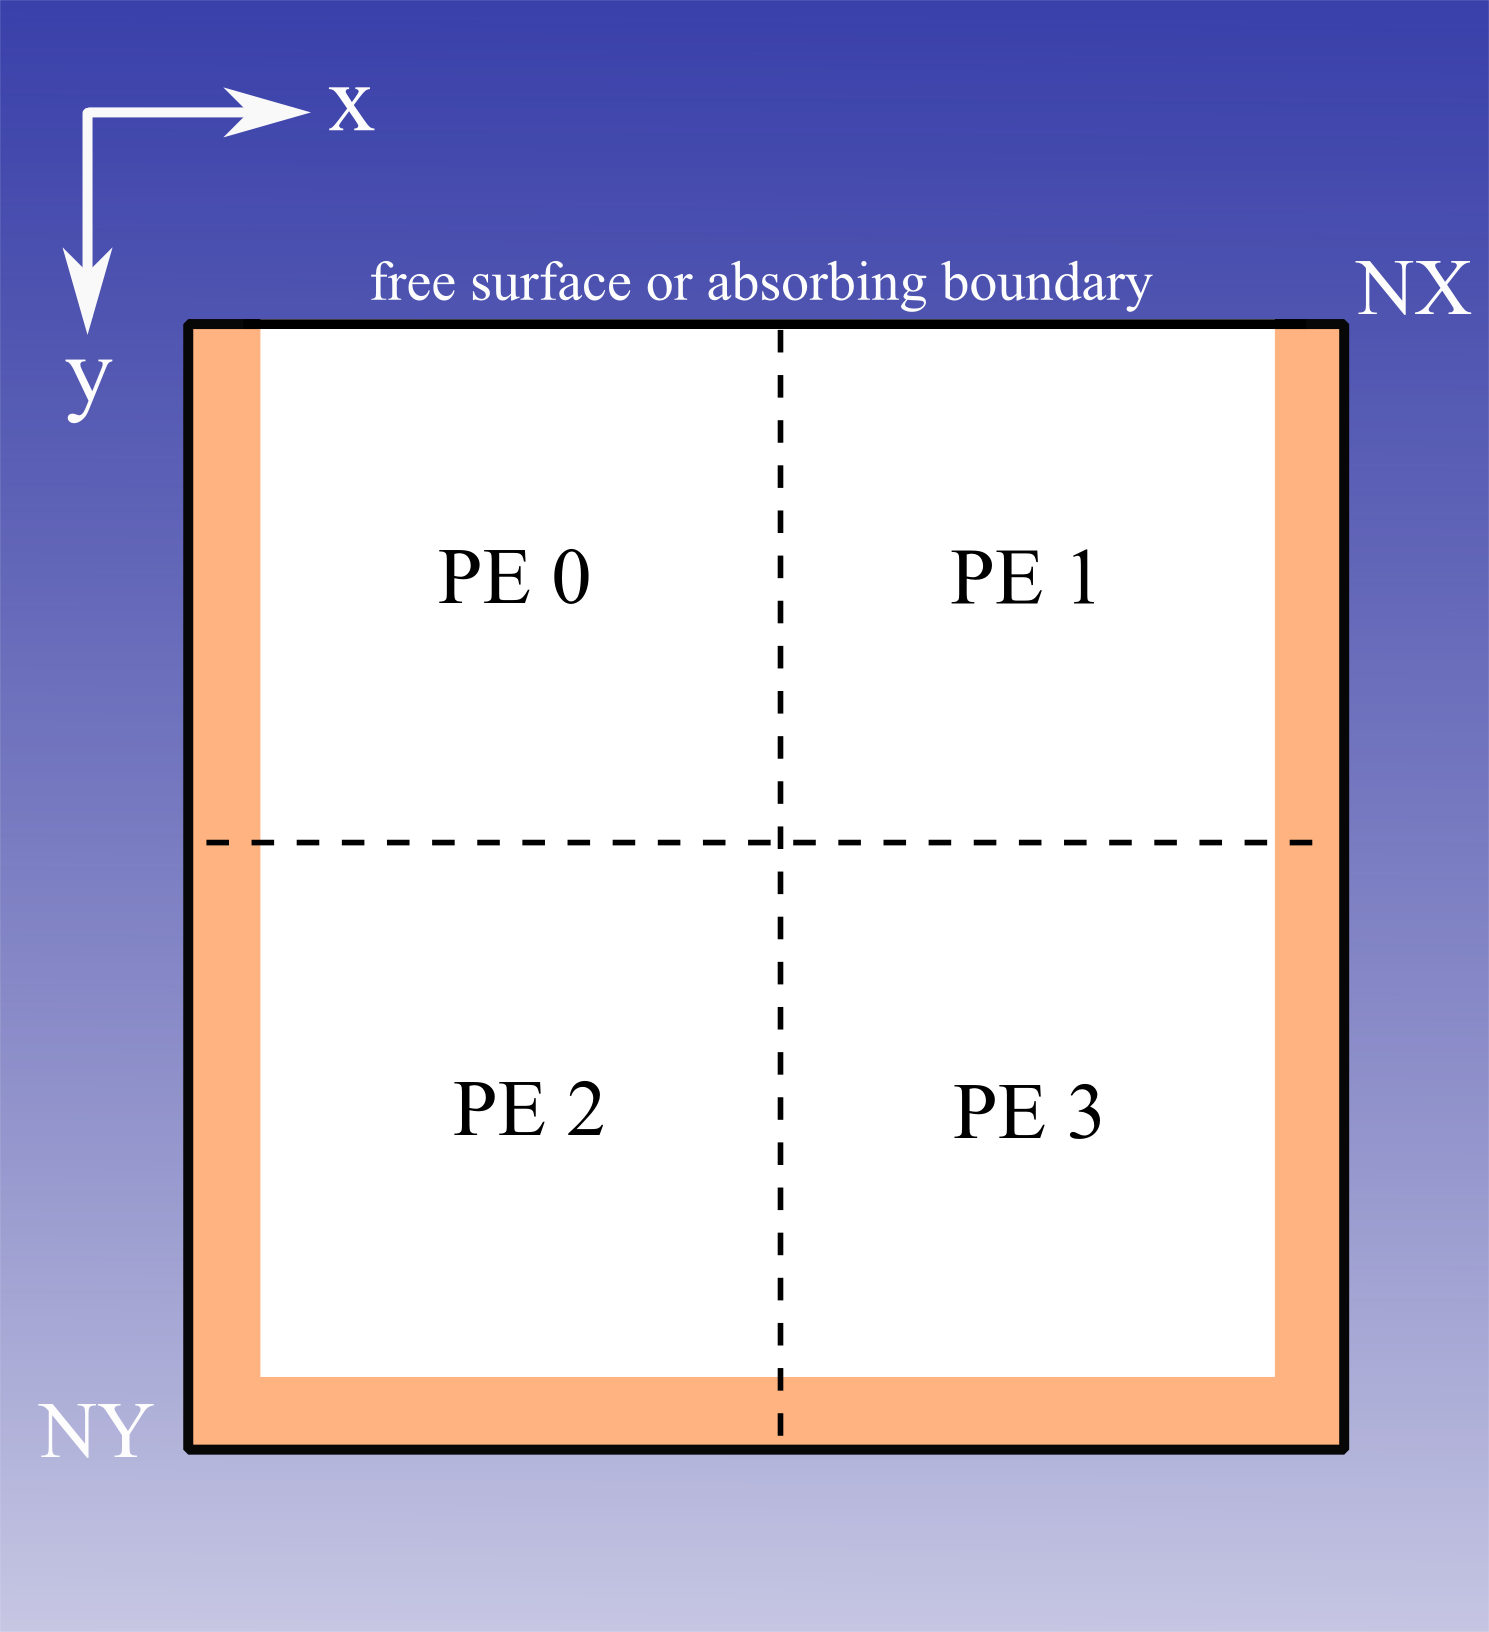
\includegraphics[width=7cm,angle=0]{figures/sketch_grid.png}
\end{center}
\caption{Geometry of the numerical FD grid using 2 processors in x-direction (NPROCX=2) and 2 processors in y-direction (NPROCY=2). Each processing element (PE) is updating the wavefield in its domain.
At the top of the numerical mesh the PEs apply a free surface boundary condition if FREE\_SURF=1, otherwise an absorbing boundary condition (PML). The width of the absorbing frame is FW grid points.  The size of the total grid is NX grid points in x-direction and NY gridpoints in y-direction. The size of each sub-grid  thus is NX/NPROCX x NY/NPROCY gridpoints. The origin of the Cartesian coordinate system (x,y) is at the top left corner of the grid.}
\label{fig_grid_json}
\end{figure}

\FloatBarrier
\newpage


\section{Order of the FD operator}
{\color{blue}{\begin{verbatim}
"FD order" : "comment",
			"FDORDER" : "2",
			"MAXRELERROR" : "0",
\end{verbatim}}}
The order of the used FD operator is defined by the option FDORDER (FDORDER=2,\,4\,6 or 8). With the option MAXRELERROR the user can switch between Taylor (MAXRELERROR=0) and Holberg (MAXRELERROR=1-4) FD coefficients of different accuracy. The chosen FD operator and FD coefficients have an influence on the numerical stability and grid dispersion (see chapter \ref{grid-dispersion}).

\section{Discretization}
{\color{blue}{\begin{verbatim}
"2-D Grid" : "comment",
			"NX" : "500",
			"NY" : "100",
			"DH" : "0.2",
\end{verbatim}}}
These lines specify the size of the total numerical grid (Figure  \ref{fig_grid_json}). NX and NY give the number of grid points in the x- and y-direction, respectively, and DH specify the grid spacing in x- and y-direction. The size of the total internal grid in meters in x-direction is NX*DH and in y-direction NY*DH. To allow for a consistent domain decomposition NX/NPROCX and NY/NPROCY must be integer values.

To avoid numerical dispersion the wavefield must be discretized with a certain number of gridpoints per wavelength. The number of gridpoints per wavelength required, depends on the order of the spatial
FD operators used in the simulation (see section \ref{grid-dispersion}). In the current FD software, 2nd, 4th, 6th and 8th order operators are implemented. The criterion to avoid numerical dispersion reads:
\begin{equation}
DH\le\frac{v_{s,\text{min}}}{2 f_c n} \label{eq_dispersion_json}
\end{equation}
where $\frac{v_{s,\text{min}}}{2 f_c}$ is the smallest wavelength propagating through the model and $v_{s,\text{min}}$ denotes the minimum shear wave velocity in the model, and $f_c=1/TS$ is the center frequency of the source wavelet. The program assumes that the maximum frequency of the source signal is approximately two times the center frequency. The center frequency is approximately one over the duration time TS. The value of n for different FD operators is tabulated in table \ref{grid_disp.2}. The criterion \ref{eq_dispersion_json} is checked by the FD software. If the criterion is violated a warning message will be displayed in the IFOS2D output section ``--- CHECK FOR GRID DISPERSION ---``. Please note, that the FD-code will NOT terminate due to grid dispersion, only a warning is given in the output file.


\section{Time stepping}
{\color{blue}{\begin{verbatim}
"Time Stepping" : "comment",
			"TIME" : "0.5",
			"DT" : "5.0e-05",
\end{verbatim}}}
The propagation time of seismic waves in the entire model is TIME (given in seconds). The time stepping interval (DT in s) has to fulfill the stability criterion \ER{courandt:1} in section \ref{courandt}. 
The program checks these criteria for the entire model, outputs a warning message if these are violated , stops the program and will output the time step interval for a stable model run. 

\newpage


\section{Sources}
\label{sec:sources}
{\color{blue}{\begin{verbatim}
"Source" : "comment",
			"SOURCE_SHAPE" : "4",
			"SOURCE_SHAPE values: ricker=1;fumue=2;from_SIGNAL_FILE=3;SIN**3=4;
			Gaussian_deriv=5;Spike=6;from_SIGNAL_FILE_in_su_format=7" : "comment",
			"SIGNAL_FILE" : "./ormsby.dat",
			
			"SOURCE_TYPE" : "3",
			"SOURCE_TYPE values (point_source): explosive=1;force_in_x=2;force_in_y=3;
			rotated_force=4" : "comment",
			
			"SRCREC" : "1",
			"SRCREC values : read source positions from SOURCE_FILE=1,
			 PLANE_WAVE=2" : "comment",
			 
			"SOURCE_FILE" : "./source/sources.dat",
			"RUN_MULTIPLE_SHOTS" : "1",
			
			"PLANE_WAVE_DEPTH" : "0.0",
			"PHI" : "0.0",
			"TS" : "0.032",
\end{verbatim}}}

{\color{red}{\begin{verbatim}
Default values are:
	SRCREC=1
\end{verbatim}}}

Five built-in wavelets of the seismic source are available. The corresponding source time functions are defined in \texttt{src/wavelet.c}. You may modify the time functions in this file and recompile to include your
own analytical wavelet or to modify the shape of the built-in wavelets.
\newline

SOURCE\_SHAPE=1, Ricker wavelet:
\begin{equation}
r(\tau)=\left(1-2\tau^2\right)\exp(-\tau^2) \quad \mbox{with} \quad \tau=\frac{\pi(t-1.5/f_c-t_d)}{1.0/f_c}
\label{eq_ricker}
\end{equation}

SOURCE\_SHAPE=2, Fuchs-M\"uller wavelet:
\begin{equation}
f_m(t)=\sin(2\pi(t-t_d)f_c)-0.5\sin(4\pi(t-t_d)f_c) \quad \mbox{if} \quad t\in[t_d,t_d+1/fc] \quad \mbox{else} \quad fm(t)=0
\label{eq_fm}
\end{equation}

SOURCE\_SHAPE=4, $sin^3$ wavelet:
\begin{equation}
s3(t)=0.75 \pi f_c \sin(\pi(t+t_d)f_c)^3\quad \mbox{if} \quad t \in[t_d,t_d+1/fc] \quad \mbox{else} \quad s3(t)=0
\label{eq_s3}
\end{equation}

SOURCE\_SHAPE=5, First derivative of a Gaussian function:
\begin{equation}
f(t)= -2.0 a (t-t_s) \exp(-a (t-t_s)^2)\quad \mbox{with} \quad a=\pi^2 f_c^2 \quad \mbox{and} \quad t_s=1.2/f_c
\label{eq_deriv_of_gaussian}
\end{equation}

SOURCE\_SHAPE=6, delta pulse: Lowpass filtered delta pulse. Note, that it is not clear if the lowpass filter used in the current version works correctly for a delta pulse.\\

% Source time function from SIGNAL\_FILE in su format (SOURCE\_SHAPE=7).\\

In these equations, t denotes time and $f_c$ is the center frequency. $t_d$ is a time delay which can be defined for each source position. Note that the symmetric (zero phase) Ricker signal is always delayed by $1.0/f_c$, which means that after one period the maximum amplitude is excited at the source location. Three of these 5 source wavelets and the corresponding amplitude spectra for a center frequency of $f_c=50$ Hz and $t_d=0$ are plotted in Figure \ref{fig_source_wavelets_json}. Note the delay of the Ricker signal described above. The Fuchs-M\"uller wavelet has a slightly higher center frequency and covers a broader frequency range.
\newline

\begin{figure}
\begin{center}
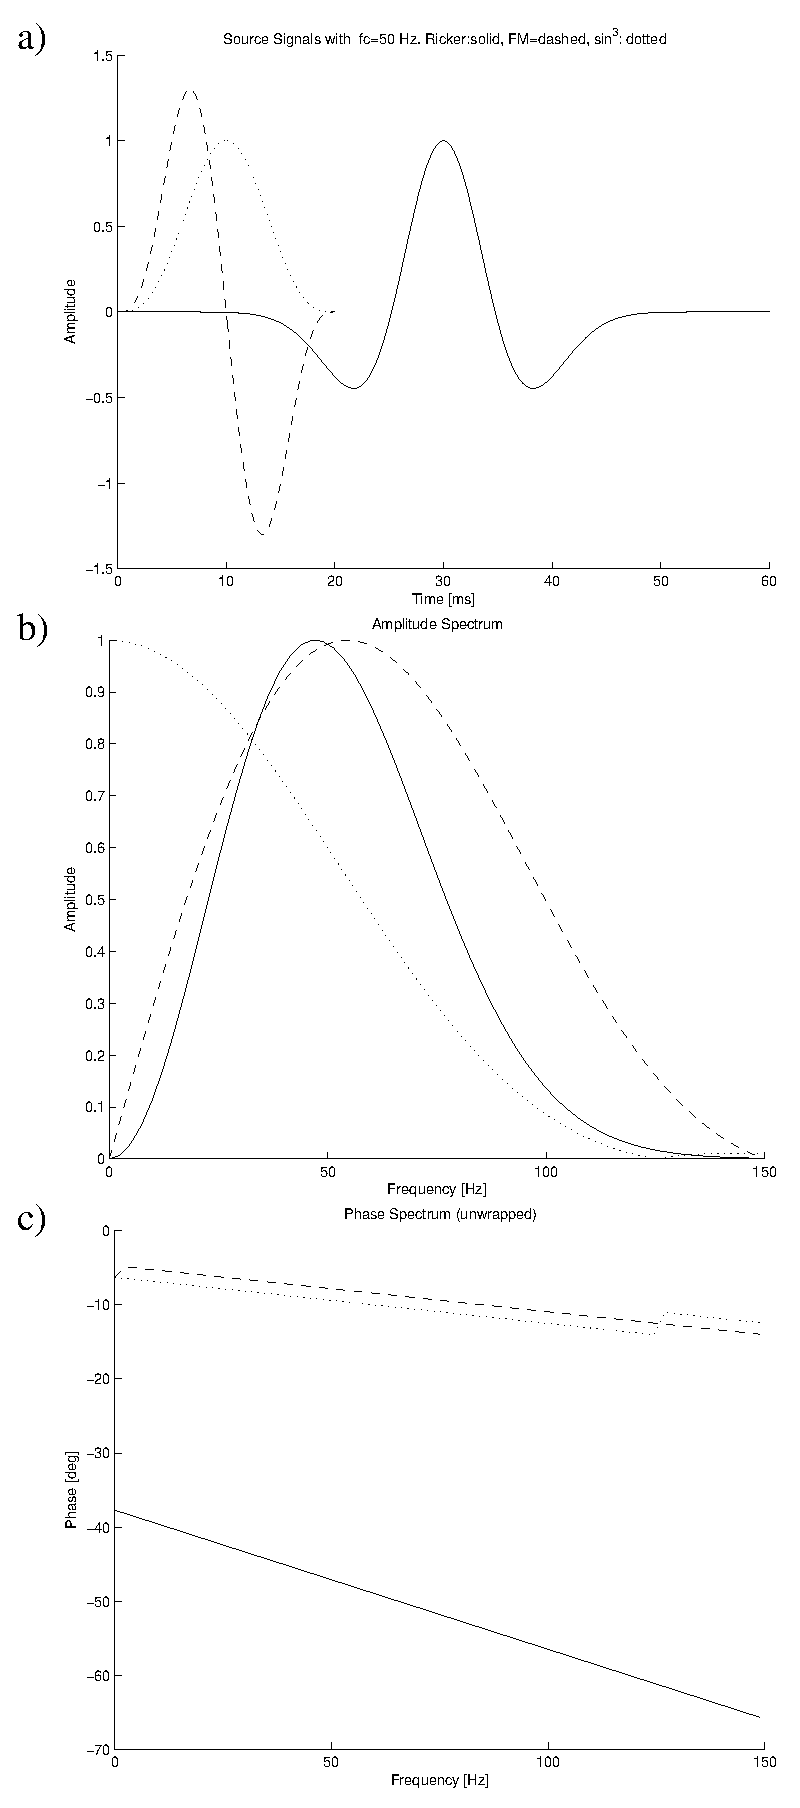
\includegraphics[width=8cm,angle=0]{figures/signals.eps}
\end{center}
\caption{Plot of built-in source wavelets (equations \ref{eq_ricker}, \ref{eq_fm}, \ref{eq_s3}) for a center frequency of $f_c=50$ Hz 
($TS=1/f_c=0.02$s): Ricker signal (solid), Fuchs-M\"uller signal (dashed), $sin^3$-signal (dotted). a) Time function, b) amplitude
spectrum, c) phase spectrum.  }
\label{fig_source_wavelets_json}
\end{figure}

\newpage

SOURCE\_SHAPE=3 allows you to use your own time function as the source wavelet stored in ASCII-format in SIGNAL\_FILE. SIGNAL\_FILE should then contain one sample per line. It should thus look like:

{\color{blue}{\begin{verbatim}
0.0
0.01
0.03
...
\end{verbatim}}}

The time interval between the samples must equal the time step interval (DT) of the FD simulation (see above)! Therefore it might be necessary to resample/interpolate a given source time function with a smaller sample rate. You may use the matlab script mfiles/resamp.m to resample your external source signal to the required sampling interval.
\newline

SOURCE\_SHAPE=7 is used for reading different external source wavelets for each shot. The wavelets in SU-format need to be saved in SIGNAL\_FILE.shot<shotnumber>.su.

If you want to use the source time function inversion (INV\_STF==1, section \ref{sec:STF}) with an external wavelet, this wavelet needs to be provided at SIGNAL\_FILE.shot<shotnumber>\_start.su and the inverted wavelets will be stored in SIGNAL\_FILE.shot<shotnumber>.su (or SIGNAL\_FILE.<workflowstage>.<shotnumber>.su if you use the WORKFLOW option).

The wavelets in each su file must have the same number of samples as specified by TIME/DT!
\newline

The following source types are availabe: explosive sources that excite compressional waves only (SOURCE\_TYPE=1), and point forces in the x- and y-direction (SOURCE\_TYPE=2,3).
The force sources excite both P- and S-waves. The explosive source is located at the same position as the diagonal elements of the stress tensor, i.e. at (i,j) (Figure \ref{fig_cell}).
The forces are located at the same position as the corresponding components of particle velocity (Figure \ref{fig_cell}). If (x,y) denotes the position at which the source location is defined in source.dat, then the actual force in x-direction is located at (x+DX/2,y) and the actual force in y-direction is located at (x,y+DY/2). With SOURCE\_TYPE=4 a custom directive force can be defined by a force angle between y and x. The angle of the force must be specified in the SOURCE\_FILE after AMP. This force is not aligned along the main directions.
\newline

The locations of multiple sources must be defined in an external ASCII file (SOURCE\_FILE) that has the following format:
{\color{blue}{\begin{verbatim}
NSRC
  % 	XSRC		ZSRC		YSRC		TD		FC		AMP  	SOURCE_AZIMUTH		SOURCE_TYPE	(NSRC lines)
\end{verbatim}}}

In the following lines, you can define certain parameters for each source point:\\
The first line must be the overall number of sources (NSRC). XSRC is the x-coordinate of a source point (in meter), YSRC is the y-coordinate of a source point (in meter). ZSRC is the z-coordinate should always be set to 0.0, because IFOS2D is a 2D code. TD is the excitation time (time-delay) for the source point (in seconds), FC is the center frequency of the source signal (in Hz), and AMP is the maximum amplitude of the source signal.
\newline

\textbf{Optional parameter:} The SOURCE\_AZIMUTH if SOURCE\_TYPE is 4. The SOURCE\_AZIMUTH is the angle between the y- and x-direction in degree and with SOURCE\_TYPE if SOURCE\_TYPE is set here, the value of SOURCE\_TYPE in the input file is ignored.

The SOURCE\_FILE = ./sources/source.dat that defines an explosive source  at $x_s=2592.0\;$ m and $y_s=2106.0\;$ m with
a center frequency of 5 Hz (no time delay) is
{\color{blue}{\begin{verbatim}
	2592.0        0.0        2106.0        0.0           5.0           1.0
\end{verbatim}}}

If the option RUN\_MULTIPLE\_SHOTS=0 in the parameter file all shot points defined in the SOURCE\_FILE are excitated simultaneously in one simulation. Setting RUN\_MULTIPLE\_SHOTS=1 will start individual model runs from i=1 to i=NSRC with source locations and properties defined at line i of the SOURCE\_FILE. (To apply a full waveform inversion you have to use RUN\_MULTIPLE\_SHOTS=1.) 

% Instead of a single source or multiple sources specified in the SOURCE\_FILE, you can also specify to excite a plane wave parallel (or tilted by an angle PHI) to the top of the model. This plane wave is approximated by a plane of single sources at every grid point at a depth of PLANE\_WAVE\_DEPTH below. The center source frequency $f_c$ is specified by the inverse of the duration of the source signal TS. SOURCE\_SHAPE and SOURCE\_TYPE are taken from the parameters as described above. If you choose the plane wave option by specifying a PLANE\_WAVE\_DEPTH$>$0, the parameters SRCREC and SOURCE\_FILE will be ignored.
% 
% This option will not be supported in future releases of IFOS2D.    

\newpage


\section{Acoustic Modelling}
\label{ac_mod}
{\color{blue}{\begin{verbatim}
"Acoustic Computation" : "comment",
			"ACOUSTIC" : "1",
\end{verbatim}}}

{\color{red}{\begin{verbatim}
Default value is:
	ACOUSTIC=0
\end{verbatim}}}

With this option pure acoustic modelling and/or inversion can be performed (ACOUSTIC = 1). Only a P-wave and a density model need to be provided. Acoustic modelling and inversion can be a quick estimate, especially for marine environments.

For acoustic modelling the option VELOCITY is not available and only PARAMETERIZATION = 1 is possible.

\section{PSV and SH modelling}
{\color{blue}{\begin{verbatim}
			"WAVETYPE" : "1",
\end{verbatim}}}

{\color{red}{\begin{verbatim}
Default value is:
	WAVETYPE=1
\end{verbatim}}}
In 2D the wave equations of PSV and SH waves are decoupled. Therefore the inversion problem is decoupled as well. With the variable WAVETYPE it is possible to switch between a PSV (WAVETYPE==1) and a SH (WAVETYPE==2) simulation. However the SH FWI is still in development and it is strongly recommended to use the PSV simulation. If ACOUSTIC is set to 1, WAVETYPE==1 will be enforced automatically.

\section{Model input}
\label{gen_of_mod}
{\color{blue}{\begin{verbatim}
"Model" : "comment",
			"READMOD" : "0",
			"MFILE" : "model/test",
\end{verbatim}}}

If READMOD=1, the P-wave, S-wave, and density model grids are read from external binary files. MFILE defines the basic file name that is expanded by the following extensions: P-wave model: ''.vp'', S-wave model: ''.vs'', density model: ''.rho''.  In the example above, the model files thus are: ''model/test.vp'' (P-wave velocity model),''model/test.vs'' (S-wave velocity model), and ''model/test.rho'' (density model). 

In these files, each material parameter value must be saved as 32 bit (4 byte) native float. Velocities must be in meter/second, density values in kg/m$^3$. The fast dimension is the y direction. See \texttt{src/readmod.c}. The number of samples for the entire model in the x-direction is NX, the number of values in the y-direction is NY. The file size of each model file thus must be NX*NY*4 bytes. You may check the model structure using the SU command ximage:
\newline

\textit{ximage n1=$<$NY$>$ $<$ model/test.vp} .
\newline

It is also possible to read Qp, and Qs grid files to allow for spatial variable attenuation. If no models are provided, the value TAU is used to generate Q-Models (see section \ref{q_approx}).

If READMOD=0 the model is generated ''on the fly'' by IFOS2D, i.e. it is generated internally before the time loop starts. See \texttt{genmod/1D\_linear\_gradient\_el.c} for an example function that generates a simple model with a linear vertical gradient ''on the fly''. If READMOD=0 this function is called in \texttt{src/IFOS2D.c} and therefore must be specified in \texttt{src/Makefile} (at the top of \texttt{src/Makefile}, see section \ref{compexec}). If you change this file, for example to change the model structure, you need to re-compile IFOS2D by changing to the src directory and ''make IFOS2D''.


\section{Free surface}  
{\color{blue}{\begin{verbatim}
"Free Surface" : "comment",
			"FREE_SURF" : "1",
\end{verbatim}}}
A plane stress free surface is applied at the top of the global grid if FREE\_SURF!=0 using the imaging method proposed by \cite{levander:88}. Note that the free surface is always located at $y$=0 or at the first grid point, respectively.


\section{Boundary conditions}
\label{abs}
{\color{blue}{\begin{verbatim}
"PML Boundary" : "comment",
			"FW" : "20",
			"VPPML" : "600.0",
			"FPML" : "31.25",
			"BOUNDARY" : "0",
			"npower" : "4.0",
			"k_max_PML" : "8.0",

\end{verbatim}}}
The boundary conditions are applied on each side face and the bottom face of the model grid. If FREE\_SURF = 0 the boundary conditions are also applied at the top face of the model grid. Note that the absorbing frames are always located INSIDE the model space, i.e. parts of the model structure are covered by the absorbing frame, in which no physically meaningful wavefield propagates. You should therefore consider the frame width when you design the model structure and the acquisition geometry (shot and receivers should certainly be placed outside).

A convolutional perfectly matched layer (CPML) boundary condition is used. The PML implementation is based on the following papers \cite{komatitsch:07} and \cite{martin:09}. A width of the absorbing frame of FW=10-20 grid points should be sufficient. For the optimal realization of the PML boundary condition you have to specify the dominant signal frequency FPML occurring during the wave simulation. This is usually the center source frequency FC specified in the source file. VPPML specifies the attenuation velocity in m/s within the PML. VPPML should be approximately the propagation velocity of the dominant wave near the model boundaries.

In some cases, it is usefull to apply periodic boundary conditions (see section \ref{bound_cond}). IF BOUNDARY=1 no absorbing boundaries are installed at the left/right sides of the grid. Instead, wavefield information is copied from left to right and vice versa. The effect is, for example, that a wave which leaves the model at the left side enters the model again at the right side.


\section{Receivers}
{\color{blue}{\begin{verbatim}
"Receiver" : "comment",
			"SEISMO" : "1",
			"READREC" : "1",
			"REC_FILE" : "./receiver/receiver.dat",
			"REFRECX, REFRECY" : "0.0 , 0.0",
			"XREC1, YREC1" : "6.0 , 0.2",
			"XREC2, YREC2" : "93.0 , 0.2",
			"NGEOPH" : "80",

\end{verbatim}}}

If SEISMO$>$0, seismograms are saved on hard disk. If SEISMO equals 1 x- and y-component of particle velocity will be written according to parameters specified in Chapter \ref{seismograms_json}.
If SEISMO = 2 pressure (sum of the diagonal components of the stress tensor) recorded at the receiver locations (receivers are hydrophones!) is written. If SEISMO = 3 the curl and divergence are saved. For SEISMO = 4 everthying is saved and for SEISMO = 5 everything except curl and divergence is saved.

The curl and divergence of the particle velocities are useful to separate between P- and S-waves in the snapshots of the wavefield. IFOS2D calculates the divergence and the magnitude of the curl of the particle velocity field according to \cite{dougherty:88}. The motivation for this is as follows. According to Morse and Feshbach \cite{morse:53} the energy of P- and S-wave particle velocities is, respectively,
\begin{equation}
E_p=\left(\lambda + 2 \mu\right) (div(\vec{v}))^2 \quad \mbox{and} \quad E_s=\mu \left|rot(\vec{v})\right|^2 \quad\mbox{.}
\label{eq_E}
\end{equation}
$\lambda$ and $\mu$ are the Lam\`{e} parameters, and $\vec{v}$ is the particle velocity vector.

The locations of the receivers may either be specified in a separate file REC\_FILE or in this parameter file. If READREC=1 receiver locations are read from the ASCII-file REC\_FILE. Each line contains the coordinates of one receiver, the first two number in each line indicate the horizontal x- and the vertical y-coordinate of each receiver position. To give an example of a receiver file, the following 3 lines specify 3 receivers located at constant depth (2106.0 m). However, the receiver coordinates change in x-direction (starting at 540 m) and therefore lining up along the x-axis. 
{\color{blue}{\begin{verbatim}
540.0   2106.0
1080.0  2106.0
1620.0  2106.0
\end{verbatim}}}
These receiver coordinates in REC\_FILE are shifted by REFREC[1], REFREC[2] into the  x- and y-direction, respectively. This allows for completely moving the receiver spread without modifying REC\_FILE. This may be useful for the simulation of moving profiles in reflection seismics.

If READREC=0 the receiver locations must be specified in the parameter file. In this case, it is assumed that the receivers are located along a straight line. The first receiver position is defined by (XREC1, YREC1), and the last receiver position by (XREC1, YREC1). The spacing between receivers is NGEOPH grid points. 

Receivers are always located on full grid indices, i.e. a receiver that is located between two grid points will be shifted by the FD program to the closest next grid point. It is not yet possible
to output seismograms for arbitrary receiver locations since this would require a certain wavefield interpolation.

\textbf{It is important to note that the actual receiver positions defined in REC\_FILE or in IFOS2D.json may vary by DH/2 due to the staggered positions of the particle velocities and stress tensor components. }

In our example, we specify 100 receiver location. Due to the small size of the model, most of the specified receiver positions will be located inside this absorbing boundary (if ABS=2, see Chapter \ref{abs}). A corresponding warning message will appear. If you choose to read the receiver location from REC\_FILE receiver.dat (READREC=1), only 10 receivers locations are considered. The list of receivers specified in file receiver.dat is equivalent to the parameters in the input file with only a larger distance between adjacent receivers (NGEOPH = 10.)


\section{Seismograms}
\label{seismograms_json}
{\color{blue}{\begin{verbatim}
"Seismograms" : "comment",
			"NDT" : "1",
			"SEIS_FORMAT" : "1",
			"SEIS_FILE" : "su/IFOS2D",
\end{verbatim}}}

{\color{red}{\begin{verbatim}
Default values are:
	NDT=1
\end{verbatim}}}

If SEISMO$>$0 seismograms recorded at the receiver positions are written to the corresponding output files. The sampling rate of the seismograms is NDT*DT seconds. In case of a small time step interval and a high number of time steps, it might be useful to choose a high NDT in order to avoid a unnecessary detailed sampling of the seismograms and consequently large files of seismogram data. Possible output formats of the seismograms are SU, ASCII and BINARY. It is recommended to use SU format for saving the seismograms. The main advantage of this format is that the time step interval (NDT*DT) and the acquisition geometry (shot and receiver locations) are stored in the corresponding SU header words. Also additional header words like offset are set by IFOS2D. This format thus facilitates a further visualization and processing of the synthetic seismograms. Note, however, that SU cannot handle sampling rates smaller than 1.0e-6 seconds and the number of samples is limited to about 32.000. In such cases, you should increase the sampling rate by increasing NDT. If this is impossible (for example because the Nyquist criterion is violated) you must choose a different output format (ASCII or binary). File endings will be added to SEIS\_FILE automatically. 


\section{Q-approximation}
\label{q_approx}
{\color{blue}{\begin{verbatim}
"Q-approximation",
			"L" : "0",
			"FL1" : "50.0", 
			"FL2" : "100.0",
			"TAU" : "0.00001",
			"F_REF" : "100",

\end{verbatim}}}

{\color{red}{\begin{verbatim}
Default values are:
	L=0
\end{verbatim}}}

These lines may be used to define an overall level of intrinsic (viscoelastic) attenuation of seismic waves. In case of L=0, a purely elastic simulation is performed (no absorption). The frequency dependence of the (intrinsic) Quality factor $Q(\omega)$ is defined by the L relaxation frequencies (FL=$f_l=2\pi/\tau_{\sigma l}$) and one value $\tau$ (see equation 5 in \cite{bohlen:02}). For a single relaxation mechanism (L=1) $Q \approx 2/\tau$ \citep{bohlen:98,blanch:95,bohlen:02}. If the model is generated ''on the fly'' the value of TAU can be assigned to all gridpoints for both P- and S-waves. Thus, intrinsic attenuation is homogeneous and equal for P- and S-waves ($Q_p(\omega)=Q_s(\omega)$). However, it is possible to simulate any spatial distribution of absorption by assigning the gridpoints with different Q-values by reading external grid files for $Q_p$ (P-waves) and $Q_s$ (S-waves) (see \texttt{src/readmod.c}) or by generating these files ''on the fly'' (see section \ref{gen_of_mod} or exemplary model function \texttt{genmod/1D\_linear\_gradient\_visc.c}).  

Small $Q$ values ($Q<50$) may lead to significant amplitude decay and velocity dispersion. Please note, that due to dispersive media properties the viscoelastic velocity model is defined for the reference frequency only. In IFOS2D, this reference frequency is specified as the center source frequency. With F\_REF one can set the reference frequency manually. At the exact reference frequency, elastic and viscoelastic models are equivalent. As a consequence, slightly smaller and larger minimum and maximum velocity values occure in the viscoelastic model.

The frequency dependence of attenuation, i.e. $Q$ and phase velocity as a function  of frequency, may be calculated using the Matlab functions in the directory mfiles. The Matlab script /mfiles/qplot.m can be used to plot $Q(\omega)$ for different values of L, $f_l$ and $\tau$. The m-file qapprox.m in the same directory finds optimal values for L, $f_l$ and $\tau$ that fit a desired function $Q(\omega)=const$ in a least-squares sense.


\section{Wavefield snapshots}
{\color{blue}{\begin{verbatim}
"Snapshots" : "comment",
			"SNAP" : "0",
			"TSNAP1" : "2.7e-3",
			"TSNAP2" : "6.0",
			"TSNAPINC" : "0.12",
			"IDX" : "1",
			"IDY" : "1",
			"SNAP_FORMAT" : "3",
			"SNAPSHOT_START , SNAPSHOT_END , SNAPSHOT_INCR" : "2, 3 , 2",
			"SNAP_FILE" : "./snap/waveform_forward",
\end{verbatim}}}

{\color{red}{\begin{verbatim}
Default values are:
SNAP=0
IDX=1
IDY=1
\end{verbatim}}}

If SNAP$>0$, wavefield information (particle velocities (SNAP=1), pressure (SNAP=2), or curl and divergence of particle velocities (SNAP=3), or everything (SNAP=4)) for the entire model is saved on the hard disk (assure that enough free space is on disk!). Each PE is writing his sub-volume to disk. The filenames have the basic filename SNAP\_FILE plus an extension that indicates the PE number in the logical processor array (SNAP\_FILE.<PEnumber>). The first snapshot is written at TSNAP1 seconds of seismic wave traveltime to the output files, the second at TSNAP1 + TSNAPINC seconds etc. The last snapshots contains wavefield at TSNAP2 seconds. With SNAPSHOT\_START (SNAPSHOT\_END) you can specify the first (last) shot, for which a snapshot should by generated. The increment for the shotwise output of the snapshots can be defined in the variable SNAPSHOT\_INCR. Note that the file sizes increase during the simulation. The snapshot files might become quite LARGE. It may therefore be necessary to reduce the amount of snapshot data by increasing IDX, IDY and/or TSNAPINC. In order to merge the separate snapshots of each PE after the completion of the wave modeling, you can use the program snapmerge (see Chapter \ref{installation}, section \textbf{src}). The bash command line to merge the snapshot files can look like this: 
\newline

\textit{../bin/snapmerge IFOS2D.json}.


\section{Monitoring the simulation}
{\color{blue}{\begin{verbatim}
"Monitoring the simulation" : "comment",
			"LOG_FILE" : "log/2layer.log",
			"LOG" : "1",
\end{verbatim}}}

{\color{red}{\begin{verbatim}
Default values are:
LOG=1
LOG_FILE="log/LOG_FILE"
\end{verbatim}}}

IFOS2D can output a lot of useful information about the modeling parameters and the status of the modeling process etc. The major part of this information is output by PE 0.
If LOG=1, PE 0 writes this info to stdout, i.e. on the screen of your shell. This is generally recommended to monitor the modeling process. You may want to save this screen info to an output file by adding ''$>$ IFOS2D.out'' or ''| tee IFOS2D.out''. to your starting command. If LOG=1 all other processes with PE number greater than zero will write their information to LOG\_FILE.<PEnumber>. If you specify LOG=2 PE 0 will also output information to LOG\_FILE.0. As a consequence only little information is written directly to the screen of your shell. On supercomputers where you submit modeling jobs to a queuing system as batch jobs LOG=2 may be advantageous. In case of LOG=2, you may still watch the simulation by checking the content of LOG\_FILE.0 for example by using the Unix commands more or tail. After finishing the program the timing information is written to the ASCII file log/test.log.0.timings. This feature is useful to benchmark your local PC cluster or supercomputer. If LOG=0 no output from node 0 will be written, neither to stdout nor to an LOG file. There will be also no output of timing information to the ASCII file log/test.log.0.timings.
If TIME\_FILT is set to one the log file L2\_LOG.dat contains a 9th column with the corner frequency in Hz used in the iteration step.

\newpage


\section{General inversion parameters}
{\color{blue}{\begin{verbatim}
"General inversion parameters" : "comment",
			"ITERMAX" : "10",
			"DATA_DIR" : "su/measured_data/IFOS2D_real",
			"PARAMETERIZATION" : "1",
			"FORWARD_ONLY" : "0",
			"ADJOINT_TYPE" : "1",
			"MISFIT_LOG_FILE" : "L2_LOG.dat",
			"VELOCITY" : "0",

"Inversion for ..." : "comment",
			"INV_RHO_ITER" : "0",
			"INV_VP_ITER" : "0",
			"INV_VS_ITER" : "0",
\end{verbatim}}}

{\color{red}{\begin{verbatim}
Default values are:
MISFIT_LOG_FILE=L2_LOG.dat
VELOCITY=0
INV_RHO_ITER=0
INV_VP_ITER=0
INV_VS_ITER=0
\end{verbatim}}}

This section covers some general inversion parameters. The maximum number of iterations is defined by ITERMAX. The switch FORWARD\_ONLY controls if only the forward modeling code should be used (FORWARD\_ONLY=1), e.\,g. to calculate synthetic seismograms or a complete FWT run (FORWARD\_ONLY=0). The seismic sections of the real data need to be located in DATA\_DIR and should have the ending \_vx.su.shot<shotnumber> for the x-component and so on. As noted in section \ref{model parametrizations} the gradients can be expressed for different model parameterizations. The switch PARAMETERIZATION defines which parameterization should be used, seismic velocities and density (Vp,Vs,rho, PARAMETERIZATION=1), seismic impedances (Zp,Zs,rho, PARAMETERIZATION=2) or Lam$\rm{\acute{e}}$ parameters ($\rm{\lambda,\mu,\rho}$, PARAMETERIZATION=3). Please use PARAMETERIZATION>1 with care, as current developers are only working with PARAMETERIZATION=1.

If models are read from binary files appropriate file extensions are required for the different models (see section \ref{gen_of_mod}). Depending on the data different components of the seismic sections can be back propagated. For two component data (x- and y-component) set ADJOINT\_TYPE=1, only the y-component (ADJOINT\_TYPE=2) and only the x-component (ADJOINT\_TYPE=3). For the inversion of pressure seismograms ADJOINT\_TYPE=4 has to be used.

During the inversion the misfit values are saved in a log file specified in MISFIT\_LOG\_FILE. The log file consists of eight or nine columns and each line corresponds to one iteration step. The used step length is written in the first column. In the second to fourth column the three test step lengths used for the step length estimation are saved. The corresponding misfit values for these test step lengthes and the test shots are written to column five to seven. Column eight corresponds to the total misfit for all shots and if you use frequency filtering then the ninth column corresponds to the corner frequency of the lowpass filter used in the inversion step.

In general IFOS2D tries to minimize the misfit in the particle displacement between the observed data and the synthetic data. If you set the switch VELOCITY to 1 the misfit in the particle velocity seismograms is minimized.

The parameters INV\_RHO\_ITER, INV\_VP\_ITER and INV\_VS\_ITER define from which inversion step on an inversion for density, Vp and Vs, respectively, is applied. To invert for one parameter from the beginning of an inversion set it to 0 or 1.


\section{Output of inversion results}
\label{sec:Output_of_inversion_results_json}
{\color{blue}{\begin{verbatim}
"Output of inverted models" : "comment",
			"INV_MODELFILE" : "model/model_Test",
			"nfstart" : "1",
			"nf" : "1",

"Output of gradients" : "comment",
			"JACOBIAN" : "jacobian/jacobian_Test",
			"nfstart_jac" : "1",
			"nf_jac" : "1",
\end{verbatim}}}

The inverted models are saved in INV\_MODELFILE. The first model that is saved is at iteration step nfstart and then every $\mathrm{nf}^{\mathrm{th}}$ iteration step. Analog the gradients are saved every $\mathrm{nf\_jac}^{\mathrm{th}}$ iteration step from iteration step nfstart\_jac on in JACOBIAN. 

\section{Workflow}
\label{sec:workflow}
{\color{blue}{\begin{verbatim}
"Workflow" : "comment",
			"USE_WORKFLOW" : "1",
			"FILE_WORKFLOW" : "workflow.txt",
\end{verbatim}}}
{\color{red}{\begin{verbatim}
Default values are:
"USE_WORKFLOW" : "0"
\end{verbatim}}}
With the use of a workflow file, you can define different FWI stages. For instance, one FWI stage could refer to one corner frequency of a low-pass filter or to a specific time window. Every line in the workflow file corresponds to one FWI stage. To use a workflow file the switch USE\_WORKFLOW have to be set to 1.  The algorithm will automatically change to the next line of the workflow file if the abort criterium of the current line is reached or if no step length could be found which reduces the misfit. The structure of the variables inside the workflow file is as follow: \\

\noindent
\begin{tabular}{llllllllllll}
\# & INV\_VS & INV\_VP & INV\_RHO & PRO & TIME\_FILT & FC & WAVETYPE & 0 & 0 & EPRECOND & EPSILON\_WE\\
\end{tabular}

\ \\
The first column is the number of the line. With INV\_* etc. you can activate the inversion for VS, VP or RHO, respectively. The abort criterium in percent for this FWI stage will be the declared in the variable PRO. With TIME\_FILT you can activate the frequency filtering with the corner frequency FC. WAVETYPE can be used to switch between PSV and SH modeling, however it is recommended to use PSV modeling (WAVETYPE==1) due to the current development on SH modeling. The following to zeros are placeholders for an upcoming update. With EPRECOND and EPSILON\_WE you can control the approx. Hessian. Please note, that all features which are used eg. TIME\_FILT (see section \ref{sec:filtering}) within the workflow have to be activated in the .JSON file.

For an example of a workflow file, have a look in the par/ folder.


\section{Approx. Hessian preconditioning}
{\color{blue}{\begin{verbatim}
			"EPRECOND" : "3",
			"EPSILON_WE" : "0.005",
			
			"EPRECOND_PER_SHOT" : "1",
\end{verbatim}}}
{\color{red}{\begin{verbatim}
Default values are:
			"EPRECOND" : "0",
\end{verbatim}}}

With the variable EPRECOND it is possible to activate an approximated Hessian for preconditioning. There are two different approximations available. EPRECOND==1 will be an approximation after \cite{shin2001efficient}, and EPRECOND==3 after \cite{plessix2004frequency}. EPSILON\_WE defines a water level to stabilize the approximated Hessian. The use of an approximated Hessian can significantly influence the speed of convergence. The Hessian is calculated for each shot individually and will be applied to the gradient from each shot directly if the switch EPRECOND\_PER\_SHOT is set to 1. Otherwise (EPRECOND\_PER\_SHOT==0) the Hessian will be summed up for each shot and will be applied to the total gradient. 
Up to now there is no rule of tumb wether EPRECOND==1 or ==3 should be chosen,  so it is recommended to try both. After each iteration the Hessian will be outputted in the folder JACOBIAN with the syntax \*approx\_hessian\* in the file name.\\
The corresponding functions are copied out of DENISE Black Edition, which is maintained by Daniel Koehn. 

\section{PCG and L-BFGS}
{\color{blue}{\begin{verbatim}
"Gradient-Method" : "comment",
			"GRAD_METHOD" : "2",
			"N_LBFGS" : "5",
			
			"WOLFE_CONDITION" : "1",
			"WOLFE_TRY_OLD_STEPLENGTH" : "1",
			"WOLFE_NUM_TEST" : "5", 
			"WOLFE_C1_SL" : "1e-4",
			"WOLFE_C2_SL" : "0.9",
			
			"LBFGS_STEP_LENGTH" : "0",
\end{verbatim}}}

{\color{red}{\begin{verbatim}
Default values are:
	"GRAD_METHOD" : "1",
\end{verbatim}}}

IFOS2D contains the option to chose between a preconditioned conjugate gradient (PCG) method or a quasi-newton L-BFGS method.

The preconditioned conjugate gradient (PCG), which can be used by GRAD\_METHOD==1, is very robust, however in general shows slow convergence. For a quick-and-dirty inversion or if you want to run an inversion without worry about a stable L-BFGS inversion it is recommended to use PCG, due to the higher stability and robustness of convergence.

The L-BFGS method is a quasi-newton method, which will implicitly approximate the Hessian and can be chosen by setting GRAD\_METHOD to 2. Therefore the differences of the models and the gradients of a N\_LBFGS last iterations will be stored. First tests showed that N\_LBFGS=10 should be enough. The L-BFGS algorithm is implemented after the book \cite{nocedal:1999}, which is recommended to be read prior to using the L-BFGS method. Prior to starting the L-BFGS method one update with steepest decent have to be done to get a first set of model and gradient differences which are necessary to start L-BFGS.

To ensure a stable convergence when L-BFGS is used the step length has to satisfy the wolf condition. A detailed description of the wolfe condition can be also found in \cite{nocedal:1999}. The first wolfe condition, which is also called sufficient decrease condition, requires that the misfit for a chosen step length will be decreased at least linear with the step length. Let $f(x)$ be the objective function, $x$ the current model, $\alpha$ the step length and $p$ the desired model update, so the first wolfe condition reads \citep{nocedal:1999}:
\begin{align}
	f(x+\alpha \cdot p) \le f(x) + c_1 \cdot \alpha \cdot\bigtriangledown f(x)^{T} \cdot p
\end{align}

The second one, which is called curvature condition, requires that the slope of the misfit function will be higher than the initial slope. This ensures that the next misfit minimum will be reached fast enough.
The second criterium is defined as \citep{nocedal:1999}:
\begin{align}
	\bigtriangledown f(x+\alpha \cdot p)^{T} \cdot p \geq c_2 \cdot\bigtriangledown f(x)^{T} \cdot p
\end{align}
To verify this condition the full gradient (with all shots!) of the updated model have to be calculated, so the verification of this condition is very expensive in terms of computation time. In theory always a step length of one should be tried first, however to save time it is possible to chose the step length from the iteration before which satisfied the wolfe condition. This behavior can be controlled with WOLFE\_TRY\_OLD\_STEPLENGTH, if this is set to 1 always the old step length will be tried first. In practice the experience has shown that at the beginning of a FWI stage a couple of step lengths will be tested and then the algorithm converges to a step length which will be accepted by the wolfe condition until the misfit cannot be reduced further. With the variable WOLFE\_NUM\_TEST a maximum number of test calculations can be defined. If after WOLFE\_NUM\_TEST tests no step length could be found, the algorithm takes the step length of the tests which reduced the misfit most, even if this step length does not satisfy the wolfe condition. If no step length was found which reduces the misfit, the algorithm will switch to the next FWI stage in the workflow file or abort the inversion. 
The variable $c_1$ will be $10^{-7}\cdot \max(f(x)^{-1}$ and $c_2$ is set to 0.9. With WOLFE\_C1\_SL and WOLFE\_C2\_SL it is possible to manipulate $c_1$ and $c_2$ with the JSON input file. If the parameters are not set, they will be set to default values, so in most cases it should be the best to do not specify theses parameters in the JSON file.
A step length search which is based on the wolfe condition can be used which the switch WOLFE\_CONDITION. Please note that this step length search is only available if GRAD\_METHOD==2. 

However, it is possible to chose a second step length search which the L-BFGS method. This one is available by the switch LBFGS\_STEP\_LENGTH=0. If you use LBFGS\_STEP\_LENGTH the wolfe condition based step length search will be deactivated automatically. Whit this search the step length 0.1, 0.5 and 1.0 will be tried and with a parabolic fit the best step length will be estimated. This search algorithm is implemented to save computation time, however the wolfe condition will not be checked, so the L-BFGS stability will not be satisfied. It is highly recommended to use the step length search based on the wolfe condition. It is likely that this option will be removed in a future releas. 


\section{Step length estimation}
{\color{blue}{\begin{verbatim}
"Step length estimation" : "comment", 
			"EPS_SCALE" : "0.01", 
			"STEPMAX" : "4",
			"SCALEFAC" : "4.0",
			"TESTSHOT_START , TESTSHOT_END , TESTSHOT_INCR" : "1 , 2 , 1",
\end{verbatim}}}

For the step length estimation a parabolic line search method proposed by \cite{sourbier:09,sourbier:09b}, \cite{brossier:2009} and \cite{nocedal:1999} is implemented. For this step length estimation only two further test forward modelings are needed. The vector L2t contains the misfit values and the vector epst contains the corresponding step length. During the forward modeling of an iteration step the misfit norm of the data residuals is calculated for the shots defined by  TESTSHOT\_START, TESTSHOT\_END and TESTSHOT\_INC. The value L2t(1) then contains the misfit from the forward modeling and the corresponding epst(1) value is 0.0.\\

The step lengths for the different parameters are defined as:\\
EPSILON = EPS\_SCALE * m\_max/grad\_max
EPSILON = epst[i] * m\_max/grad\_max\\
where m\_max is the maximum value of the corresponding model parameter in the whole model and grad\_max is the maximum absolute value of the gradient.\\

For a better definition of the parabola the improved line search is now trying to estimate a steplength epst(2) with L2t(2)<L2t(1). If the code is not able to find an appropiate steplength using the user-defined value EPS\_SCALE (f.e. EPS\_SCALE = 0.01 = 1\% change in terms of m\_max/grad\_max), the code divides this steplength by the variable SCALEFAC and calculates the misfit norm again. If this search fails after STEPMAX attempts IFOS2D exits with an error message. If the algorithm has found an appropriate value for epst(2), it is trying to estimate a steplength epst(3) with L2t(3)> L2t(2), by increasing the steplength\\

EPS\_SCALE += EPS\_SCALE/SCALEFAC.\\

If a corresponding value epst(3) can be found after STEPMAX forward modellings, IFOS2D can fit a parabola through the 3 points (L2t(i),epst(i)) and estimates an optimum step length at the minimum of the parabola. If the L2-value L2t(3) after STEPMAX forward models is still smaller than L2t(2) the optimum steplength estimated by parabolic fitting will be not larger than epst(3).\\

Please note: This step length search is only available wenn PCG method (GRAD\_METHOD==1) is used and will be automatically selected.


\section{Misfit definition}
{\color{blue}{\begin{verbatim}
"Misfit Definition" : "comment",
			"LNORM" : "2",
			"NORMALIZE" : "0",
			"DTINV" : "2",
			"WATERLEVEL_LNORM8" : "0.0",
\end{verbatim}}}

With LNORM=2 the L2 norm is used as misfit definition. In this case the misfit is scaled with the energy of the observed seismograms.\\
With LNORM=5 the global correlation is used as misfit function. It was suggested e.\,g. by \cite{choi:2012} and consists of a zero-lag cross correlation of two normalized signals. The misfit is calculated by
\begin{equation}
E = - \sum_i^{ns} \sum_j^{nr} \sum_k^{nc} \frac{\vec{u}_{i,j,k} \cdot \vec{d}_{i,j,k}}{|\vec{u}_{i,j,k}| |\vec{d}_{i,j,k}|}
\end{equation}
where the sum over $i$ denotes the sum over the sources, the sum over $j$ denotes the sum over the receivers and the sum over $k$ denotes the sum over the components used in the inversion. $\vec{u}$ are the forward modeled data and $\vec{d}$ are the observed data. The misfit is minimized but the misfit function is not yet normalized. Therefore, a perfect fit results in a misfit of $(-1)\cdot ns \cdot nr \cdot nc$.\\
LNORM=1 uses the L1 norm, LNORM=3 the Cauchy norm and LNORM=4 the SECH norm.\\
LNORM=7 uses the normalized L2 norm
\begin{equation}
 E=\frac{\sum_i^{ns} \sum_j^{nr} \sum_k^{nc} \left| \frac{\vec{u}_{i,j,k}}{|\vec{u}_{i,j,k}|}-\frac{\vec{d}_{i,j,k}}{|\vec{d}_{i,j,k}|}\right|^2}{\sum_i^{ns} \sum_j^{nr} \sum_k^{nc} \left| \frac{\vec{d}_{i,j,k}}{|\vec{d}_{i,j,k}|}\right|^2}
\end{equation}
 suggested by \cite{choi:2012}. The misfit is scaled with the energy of the observed seismograms.\\ 
LNORM=8 is based on an envelope-based objective function which compares the difference between the envelopes of observed and synthetic wave fields.
The misfit function is defined by
\begin{equation}
E= \frac{1}{2} \sum_i^{ns} \sum_j^{nr} \sum_k^{nc} \int_0^T \left( \text{env}(\vec{u}_{i,j,k}) - \text{env}(\vec{d}_{i,j,k}) \right)^2~\text{d}t.
\label{misfit_envelope}
\end{equation}
At time samples $t$ where the envelope of the synthetics $\text{env}( u)$ becomes small with respect to the noise of the observed data $\text{env}( d)$, the corresponding adjoint source develops a singularity (for $\text{env}( u) \rightarrow 0$). A finite water-level (WATERLEVEL\_LNORM8) is used to keep the division regular. The water-level is estimated about the smallest signal amplitude of the observed data which is considered in the misfit.\\
If NORMALIZE is set to 1, the synthetic data and the measured data will be normalized before calculating the residuals.\\

To reduce the memory requirements during an inversion one can define that only every DTINV time sample is used for the calculation of the gradients. To set this parameter appropriately one has to keep in mind the Nyquist criterion to avoid aliasing effects.


\section{Abort criterion}
\label{json:abort_criterion}
{\color{blue}{\begin{verbatim}
"Termination of the programmme" : "comment",
			"PRO" : "0.01",
\end{verbatim}}}
Additionally to the parameter ITERMAX a second abort criterion is implemented in IFOS2D which is using the relative misfit change within the last two iterations. The relative misfit of
the current iteration step and the misfit of the second to last iteration step is calculated with regard to the misfit of the second to last iteration step. If this relative change is
smaller than PRO the inversion aborts or in case of using frequency filtering (TIME\_FILT==1) it increases the corner frequency of the low pass filter and therefore switches to next higher bandwidth. 

\newpage

\section{Source wavelet inversion}
\label{sec:STF}
To remove the contribution of the unknown source time function (STF) from the waveform residuals, it is necessary to design a filter which minimizes the misfit to the field recordings and raw synthetics. Therefore, a second forward simulation is applied. The first one is done with the wavelet specified in SOURCE\_SHAPE and the second one with the optimized source wavelet saved in SIGNAL\_FILE (see Section~\ref{sec:sources}). This optimized source wavelet is kept constant within N\_STF or within a frequency range (see below).\\

{\color{blue}{\begin{verbatim}
"Definition of inversion for source time function" : "comment",
			"INV_STF" : "0",
			"PARA" : "fdlsq:exp=1.0",
			"N_STF" : "10",
			"N_STF_START" : "1",
			"TAPER_STF" : "0",
			"TRKILL_STF" : "0", 
			"TRKILL_FILE_STF" : "./trace_kill/trace_kill",
\end{verbatim}}}

{\color{red}{\begin{verbatim}
Default values are:
	INV_STF=0
\end{verbatim}}}

INV\_STF should be switched to 1 if you want to invert for the source time function.
\newline

An example for the parameter string provided in PARA is:
\begin{itemize}
 \item To select frequency domain least squares (fdlsq), apply offset dependent weights and a waterlevel use\\
 \textit{fdlsq:exp=1.0:waterlevel=0.01}
\end{itemize}

In most cases the frequency domain least squares engine is the best approach to find a suitable wavelet. There are also other possibilities, if you want to use those a detailed look at the libraries and the acompanying documentation provided in the folder /contrib is recommended. Here only the two main parameters for the fdlsq approach are described.

Due to the amplitude decay with offset to the source signals from receivers at larger offset would contribute less to the optimization criterion for which the source wavelet correction filter is constructed. The option exp=k provides means to add a weight factor $(r/1\text{m})^k$ to each signal, where r is the receiver to source offset. This is used to compensate the decrease in signal amplitude.

The procedure is implemented in the Fourier domain. Fourier coefficients for the correction filter are constructed such that the residual between Fourier coefficients of recorded signals and Fourier coefficients of synthetic signals after application of the correction filter are minimized in a least-squares sense. The least-squares solution is subject to a damping constraint. If the weighted power spectral density of the synthetics at a given frequency drops below the l-th fraction (waterlevel parameter) of the average (over all frequencies) power spectral density, the filter coefficients are damped (artificially made smaller) by the damping constraint (i.e. waterlevel as seen from the perspective of deconvolution). 

Start with l=0.01 as a reasonable initial value for the waterlevel. The best fitting waterlevel must be searched by trial and error and depends of signal noise and on how well the synthetics describe the actually observed wave propagtion.

The theory behind the Fourier domain least squares procedure is outlined by Lisa Groos (2013, Appendix F, page 146). She also describes a way to find an approrpiate waterlevel by application of the L-curve criterion (Groos, 2013, Appendix G, page 148).
\newline

N\_STF is the increment between the iteration steps. N\_STF\_START defines at which iterationstep the inversion for STF should start. This parameter has to be set at least to 1 NOT(!) 0. When using TAPER\_STF = 1, the source signal is tapered. See \texttt{src/taper.c} for the taper definition. With TRKILL\_STF = 1 it is possible to apply a trace killing for the estimation of the source wavelet correction filter (see section \ref{sec:trace_killing}).
\newline

Please note: If you additionally switch on frequency filtering during the inversion (TIME\_FILT=1 or TIME\_FILT=2), the parameters N\_STF and N\_STF\_START will be ignored. But the optimal source time function will be inverted for the first iteration and after every change of the frequency range.

For more information see chapter \ref{cha:STF-Inversion}.


\section{Data manipulation}
\subsection{Frequency filtering}
\label{sec:filtering}
{\color{blue}{\begin{verbatim}
"Frequency filtering during inversion" : "comment",
			"TIME_FILT" : "0",
			"F_HP" : "1",
			"FC_START" : "10.0",
			"FC_END" : "75.0",
			"FC_INCR" : "10.0",
			"ORDER" : "2",
			"ZERO_PHASE" : "0",
			"FREQ_FILE"  : "frequencies.dat",
			"WRITE_FILTERED_DATA" : "0",
			
			"Minimum number of iteration per frequency" : "comment",
			"MIN_ITER" : "10",
\end{verbatim}}}

{\color{red}{\begin{verbatim}
Default values are:
	TIME_FILT=0
	ZERO_PHASE=0
	MIN_ITER=0
\end{verbatim}}}

TIME\_FILT = 1 can be set to use frequency filtering. The parameter FC\_START defines the corner frequency of the Butterworth low pass filter at the beginning of the inversion. The parameter FC\_END defines the maximum corner frequency used in the inversion. The parameter FC\_INCR controls in which steps the bandwidth is increased during the inversion.

If TIME\_FILT = 2 individual frequencies for each step can be read from FREQ\_FILE. In this file the first entry must be the number of frequencies used for filtering. Each frequency in Hz has to be specified in a row. The example file frequencies.dat can be found in \texttt{trunk/par}.

The parameter ORDER defines the order of the Butterworth low pass filter. If the variable ZERO\_PHASE is set to one a zero phase filter is applied. It is realized by filtering the traces in both forward and reverse direction with the defined Butterworth low pass filter. Therefore, the effective order of the low pass filter is doubled. 

With F\_HP an additional high pass filter can be applied, where F\_HP is the corner frequency in Hz.

With the parameter PRO (see~\ref{json:abort_criterion}) one has to adjust the criterion that defines at which points the bandwidth of the signals are increased.

With the parameter WRITE\_FILTERED\_DATA it is possible to write the time filtered measured data to disk which are filtered with the same filter as the synthetic data. Therefore this output can be used to visualize the residuals between synthetic and measured data. The filtered data is located in DATA\_DIR and are labeled with "\_measured".

If you are using frequeny filtering (TIME\_FILT==1) during the inversion, you can set a minimum number of iterations per frequency. Within this minimum number of iteration per frequency the abort criterion PRO will receive no consideration.

\subsection{Time windowing}
{\color{blue}{\begin{verbatim}
"Time windowing" : "comment",
			"TIMEWIN" : "0",
			"TW_IND" : "0",
			"PICKS_FILE" : "./picked_times/picks"
			"TWLENGTH_PLUS" : "0.01",
			"TWLENGTH_MINUS" : "0.01",
			"GAMMA" : "100000",
\end{verbatim}}}

{\color{red}{\begin{verbatim}
Default values are:
	TIMEWIN=0
\end{verbatim}}}

To apply time windowing in a time series the paramter TIMEWIN must set to 1. A automatic picker routine is not integrated. The point in time (picked time) for each source must be specified in separate files. The folder and file name can be set with the parameter PICKS\_FILE. The files must be named like this PICKS\_FILE\_<sourcenumber>.dat. So the number of sources must be equal to the number of files. Each file must contain the picked times for every receiver.

The parameters TWLENGTH\_PLUS and TWLENGTH\_MINUS specify the length of the time window after (PLUS) and before (MINUS) the picked time. The unit is seconds. The damping factor GAMMA must be set individually.

When usig TW\_IND = 1 three columns are expected in PICK\_FILE for each trace with the picked time, time window length plus and time window length minus. In this case TWLENGTH\_PLUS and TWLENGTH\_MINUS are ignored.

If you use the option "Workflow" (section \ref{sec:workflow}) it is possible to define separate files for each workflow stage. They have to be named PICKS\_FILE\_<sourcenumber>\_<workflowstage>.dat. If you don't provide separate files for some or all stages the standard file (PICKS\_FILE\_<sourcenumber>.dat) is used. This means a standard file should exist in any case.

\subsection{Trace killing}
\label{sec:trace_killing}
{\color{blue}{\begin{verbatim}
"Trace killing" : "comment",
			"TRKILL" : "0",
			"TRKILL_FILE" : "./trace_kill/trace_kill",
			
			"TRKILL_OFFSET" : "0",
			"TRKILL_OFFSET_LOWER" : "20",
			"TRKILL_OFFSET_UPPER" : "100",
\end{verbatim}}}

{\color{red}{\begin{verbatim}
Default values are:
	TRKILL=0
\end{verbatim}}}

If you don't want to use single traces or a subset of your data, the parameter TRKILL can be used. If it is set to 1, trace killing is in use. The necessary file can be selected needs to be located at TRKILL\_FILE.dat. The file should include a kill table, where the number of rows is the number of receivers and the number of columns reflects the number of sources. Now, a 1 (ONE) means, YES, please kill the trace. The trace is NOT used, it should be killed. A 0 (ZERO) means, NO, this trace should NOT be killed. 

If you use the option "Workflow" (section \ref{sec:workflow}) it is possible to define separate files for each workflow stage. They have to be named TRKILL\_FILE\_<workflowstage>.dat. If you don't provide separate files for some or all stages the standard file (TRKILL\_FILE.dat) is used. This means a standard file should exist in any case.

Moreover, you can directly define a offset range that should be killed. Simply set TRKILL\_OFFSET and TRKILL to one and all traces with a offset between TRKILL\_OFFSET\_LOWER and TRKILL\_OFFSET\_UPPER will be killed.

\section{Gradient manipulation}
\subsection{Definition of a gradient taper}
\label{sec:Definition_of_gradient_taper_geometry}
{\color{blue}{\begin{verbatim}
"Definition of gradient taper geometry" : "comment",
			"SWS_TAPER_GRAD_VERT" : "0",
			"SWS_TAPER_GRAD_HOR" : "0",
			"GRADT1 , GRADT2 , GRADT3 , GRADT4" : "5 , 15 , 490 , 500",
			"SWS_TAPER_GRAD_SOURCES" : "0",
			"SWS_TAPER_CIRCULAR_PER_SHOT" : "0",
			"SRTSHAPE" : "1",
			"SRTRADIUS" : "5.0",
			"FILTSIZE" : "1",
			"SWS_TAPER_FILE" : "0",
			"SWS_TAPER_FILE_PER_SHOT" : "0",
			"TAPER_FILE_NAME" : "taper",
\end{verbatim}}}

{\color{red}{\begin{verbatim}
Default values are:
SWS_TAPER_GRAD_VERT=0
SWS_TAPER_GRAD_HOR=0
SWS_TAPER_GRAD_SOURCES=0
SWS_TAPER_CIRCULAR_PER_SHOT=0
SWS_TAPER_FILE=0
SWS_TAPER_FILE_PER_SHOT=0
\end{verbatim}}}

Different preconditioning matrices can be created and applied to the gradients (using the function \texttt{taper\_grad.c}). To apply a vertical taper one has to set the switch SWS\_TAPER\_GRAD\_VERT to one and for a horizontaltaper SWS\_TAPER\_GRAD\_HOR has to be 1. The parameters for the vertical and the horizontal window are defined by the input file paramters GRADT1, GRADT2, GRADT3 and GRADT4. Please have a look at the function \texttt{taper\_grad.c} directly to obtain more information about the actual definition of the tapers. It is also possible to apply cylindrical tapers around the source positions. This can be done by either setting the switch SWS\_TAPER\_GRAD\_SOURCES or SWS\_TAPER\_CIRCULAR\_PER\_SHOT to 1. If one uses SWS\_TAPER\_GRAD\_SOURCES=1 only the final gradients (that means the gradients obtained by the summation of the gradients of each shots) are multiplied with a taper that decreases the gradients at all shot positions. Therefore, one looses the update information at the source positions. To avoid this one can use SWS\_TAPER\_CIRCULAR\_PER\_SHOT=1. In this case the gradients of the single shots are preconditioned with a window that only decreases at the current shot position. This is done before the summation of all gradients to keep model update information also at the shot positions. The actual tapers are generated by the function \texttt{taper\_grad.c} and \texttt{taper\_grad\_shot.c}, respectively. The circular taper around the source positions decrease from a value of one at the edge of the taper to a value of zero at the source position. The shape of the decrease can be defined by an error function (SRTSHAPE=1) or a log-function (SRTSHAPE=2). The radius of the taper is defined in meter by SRTRADIUS. Note, that this radius must be at least 5 gridpoints. With the parameter FILTSIZE one can extend the region where the taper is zero around the source. The taper is set to zero in a square region of (2*FILTSIZE+1 times 2*FILTSIZE+1) gridpoints. All preconditioning matrices that are applied are saved in the par directory with the file names taper\_coeff\_vert.bin, taper\_coeff\_horz.bin and taper\_coeff\_sources.bin.\\

To apply an externally defined taper on the gradients in IFOS2D, the parameter SWS\_TAPER\_FILE has to be set to 1. Each model parameter requires a taper file which needs to be located in TAPER\_FILE\_NAME.vp for vp, in TAPER\_FILE\_NAME.vs for vs and in TAPER\_FILE\_NAME.rho for the density.\\

It is also possible to apply externally defined taper files to the gradients of the single shots before summation of these gradients. This can be done by setting SWS\_TAPER\_FILE\_PER\_SHOT to one. IFOS2D expects the tapers in TAPER\_FILE\_NAME.shot<shotnumber>.vp for the vp gradients, in TAPER\_FILE\_NAME.shot<shotnumber>.vs for the vs gradients and in TAPER\_FILE\_NAME.shot<shotnumber>.rho for the density gradients.\\

If you use the option "Workflow" (section \ref{sec:workflow}) it is possible to define separate files for each workflow stage. They have to be named TAPER\_FILE\_NAME(.shot<shotnumber>)\_<workflowstage>.vp etc. If you don't provide separate files for some or all stages the standard file (TAPER\_FILE\_NAME(.shot<shotnumber>).vp etc.) is used. This means a standard file should exist in any case.

\subsection{Spatial filtering of the gradients}
{\color{blue}{\begin{verbatim}
"Definition of smoothing (spatial filtering) of the gradients" : "comment",
			"SPATFILTER" : "0",
			"SPAT_FILT_SIZE" : "40",
			"SPAT_FILT_1" : "1",
			"SPAT_FILT_ITER" : "1",
\end{verbatim}}}

{\color{red}{\begin{verbatim}
Default values are:
	SPATFILTER=0
\end{verbatim}}}

One can apply a spatial Gaussian filter to the gradients that acts in horizontal direction (SPATFILTER=1). Have a look at the function \texttt{spat\_filt.c} for more information.

\subsection{Smoothing the gradients}
{\color{blue}{\begin{verbatim}
"Definition of smoothing the gradients with a 2D-Gaussian filter" : "comment",
                        "GRAD_FILTER" : "0",
                        "FILT_SIZE_GRAD" : "5",
			"GRAD_FILT_WAVELENGTH" : "0",
			"A" : "0.0",
\end{verbatim}}}

{\color{red}{\begin{verbatim}
Default values are:
	GRAD_FILTER=0
	GRAD_FILT_WAVELENGTH=0
\end{verbatim}}}

If GRAD\_FILTER = 1 the gradients are smoothed with a 2D median filter after every iterationstep. With FILT\_SIZE\_GRAD you can set the filter length in gridpoints.\\
For GRAD\_FILT\_WAVELENGTH = 1 (and TIME\_FILT=1) a new wavelength dependent filter size for smoothing the gradients is calculated by
\begin{equation}
 \mbox{FILT\_SIZE\_GRAD} = \frac{V_{s,\text{average}}\cdot \text{A}}{\text{FC}}
\end{equation}
where FC is the corner frequency of TIME\_FILT and A is a weighting factor.


\section{Model manipulation}
\subsection{Limits for the model parameters}
{\color{blue}{\begin{verbatim}
"Upper and lower limits for model parameters" : "comment",
			"VPUPPERLIM" : "3500",
			"VPLOWERLIM" : "0",
			"VSUPPERLIM" : "5000",
			"VSLOWERLIM" : "0",
			"RHOUPPERLIM" : "5000",
			"RHOLOWERLIM" : "0",
\end{verbatim}}}

{\color{red}{\begin{verbatim}
Default values are:
VPUPPERLIM=25000.0
VPLOWERLIM=0.0
VSUPPERLIM=25000.0
VSLOWERLIM=0.0
RHOUPPERLIM=25000.0
RHOLOWERLIM=0.0
\end{verbatim}}}

The six limits for the model parameters specify the minimum and maximum values which may be achieved by the inversion. Here, known a priori information can be used. Depending on the choice of the parameter PARAMETERIZATION, either vp and vs or lambda and mu is meant.

\subsection{Limited update of model parameters}
{\color{blue}{\begin{verbatim}
"Limited model update in reference to the starting model" : "comment",
"S" : "0",
"S_VS" : "0.0",
"S_VP" : "0.0",
"S_RHO" : "0.0",
\end{verbatim}}}
{\color{red}{\begin{verbatim}
Default values are:
	S=0
\end{verbatim}}}
For S=1 individual limited updates of the elastic model parameters are considered. S\_VS, S\_VP and S\_RHO are the maximum updates of the model parameters at each grid point (given in \%) in reference to the model parameters of their starting models for S-wave and P-wave velocity as well as density, respectively. For example S\_VS = 30.0 means that the model parameter update of the S-wave velocity model is limited to 30\,\% at each grid point in reference to the starting model of the S-wave velocity model. Zero (S\_VS=0.0, S\_VP=0.0 or S\_RHO=0.0) means that the model parameter won't be updated at all. S\_VS=100.0, S\_VP=100.0 or S\_RHO=100.0 equal to S=0.

\subsection{Vp/Vs ratio}
{\color{blue}{\begin{verbatim}
"Minimum Vp/Vs-ratio" : "comment",
"VP_VS_RATIO" : "1.5",
\end{verbatim}}}
{\color{red}{\begin{verbatim}
Default values are:
	VP_VS_RATIO > 1
\end{verbatim}}}
With VP\_VS\_RATIO = 1.5 (e.g.) it is possible to ensure a minimum Vp/Vs ratio during the inversion. This is done by checking the Vp/Vs ratio at every grid point after every model update and if it is less than (e.g.) 1.5 the P-wave velocity will be increased. For smaller values than one (1) this criterion is disregarded.

\subsection{Smoothing the models}
{\color{blue}{\begin{verbatim}
"Definition of smoothing the models vp and vs" : "comment",
			"MODEL_FILTER" : "0",
			"FILT_SIZE" : "5",
\end{verbatim}}}

{\color{red}{\begin{verbatim}
Default values are:
	MODEL_FILTER=0
\end{verbatim}}}

If MODEL\_FILTER = 1 vp- and vs-models are smoothed with a 2D median filter after every iterationstep. With FILT\_SIZE you can set the filter length in gridpoints.